\documentclass[a4paper, ngerman]{article}
\usepackage[ngerman]{babel}
\usepackage[ngerman]{isodate}
%\usepackage[T1]{fontenc}
%\usepackage{selinput} 
\usepackage[utf8]{inputenc}
\usepackage{parskip}
\usepackage{csquotes}
\usepackage{booktabs}
\usepackage{amsmath}
\usepackage{graphicx}
\usepackage{tikz}
\usepackage{pgfplots}
\usepackage{fancyhdr}
\usepackage{titling}
\usepackage{lastpage}
\usepackage{tabularx}
\usepackage[Q=yes]{examplep}
\usepackage[toc,page]{appendix}
\usepackage{a4wide}
\usepackage{multirow}
\usepackage{hyperref}
\usepackage{rotating}
\usepackage{scrextend}
\usepackage{framed}
\usepackage[os=win]{menukeys}
\usepackage{framed}
\usepackage{float}

%\usepackage[linguistics]{forest}

\pgfplotsset{compat=newest}


\newenvironment{command}{
	\begin{leftbar}
	}
	{
		\vspace{0.5em}
	\end{leftbar}
}


\author{Christoph Holzinger \\Raphael Kapeller \\Georg Krautinger \\Jürgen Kühnl \\Niklas Lirscher }

\title{Übung 9: NAT – HSRP/VRRP}

\date{\origdate\today}



\pagestyle{fancy}

\fancyhf{}


\lhead{\thetitle}

\lfoot{Gruppe 1a - 2a}
\rfoot{Seite \thepage\ von \pageref{LastPage}}

\renewcommand{\headrulewidth}{1pt}
\renewcommand{\footrulewidth}{1pt}
\renewcommand{\familydefault}{\sfdefault}

\renewcommand{\appendixname}{Anhang}
\renewcommand{\appendixpagename}{Anhänge}
\renewcommand{\appendixtocname}{Anhänge}


\pretitle{\begin{center}\huge}

\posttitle{\par\end{center}\vskip 0.5em}

\preauthor{\begin{center}

	\large \lineskip 0.5em%

	\begin{tabular}[t]{c}}

\postauthor{\end{tabular}\par\end{center}}

\predate{\begin{center}\normalsize\bigskip Netzwerktechnik \\\smallskip 2021/22 \textbar{} }

\postdate{\par\end{center}}

\begin{document}

\begin{titlingpage}

    \maketitle

    \vspace{60pt}

    \begin{center}
        Fehlend: \\
        Timon Babinger \\
        Erik Hakobyan \\
        Clemens Haidinger \\
        Zhe Lei
    \end{center}

    \vfill

    \vspace{-100pt}

    \begin{center}

        \begin{tabbing}

            Übungsdatum \quad \= \kill

            Klasse \> 4AHITN \\

            Gruppe \> 1a - 2a \\

            Übungsdatum \> \origdate{21.02.2022} \\[20pt]
            %			Übungsdatum \> \origdate\daterange{29.11.2019}{29.11.2019} \\[20pt]

        \end{tabbing}

    \end{center}

\end{titlingpage}



\tableofcontents

\newpage

\section{Netzaufbau}

\begin{figure}[H]
    \centering
    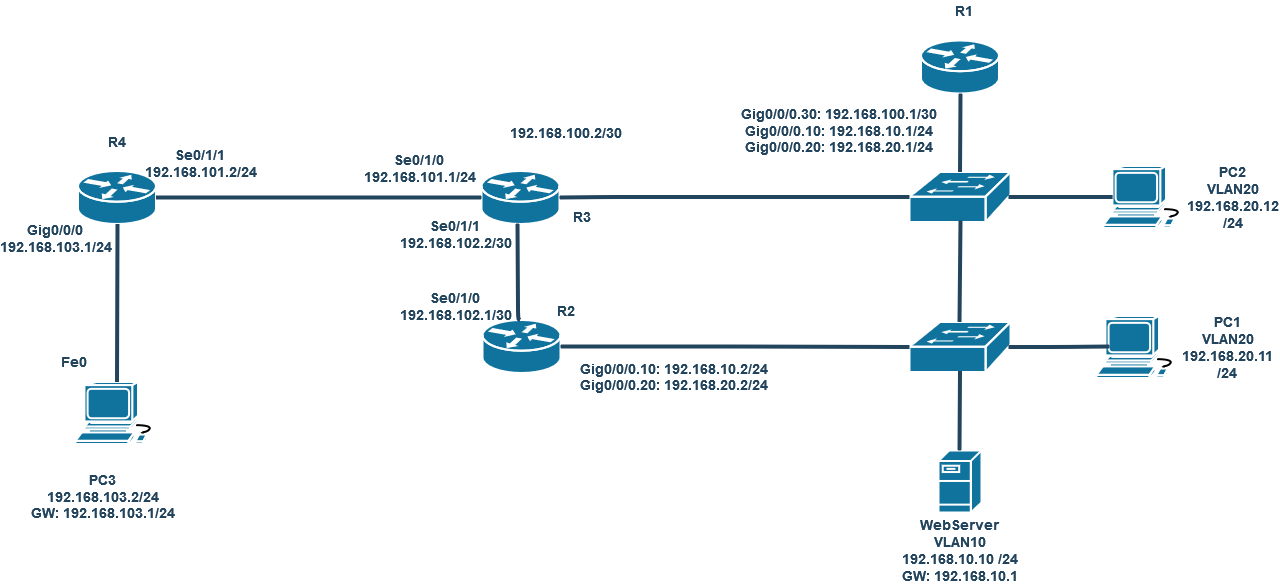
\includegraphics[scale=0.32]{screenshots/netzplan.png}
    \caption{Netzplan}
\end{figure}

\subsection{Gerätezuteilung}

Für eine besser Übersicht über die Bezeichnung im Netzplan und den Bezeichnungen der realen Geräten haben wir folgende Tabelle erstellt:

\begin{table}[ht]
    \caption{Gerätezuteilung} % title of Table
    \centering % used for centering table
    \begin{tabular}{c c} % centered columns (4 columns)
        \hline\hline
        \\
        \textbf{Bezeichnung Netzplan} & \textbf{Reales Gerät} \\ [0.5ex]
        \hline
        R1                            & R050                  \\ % inserting body of the table
        R2                            & R060                  \\
        R3                            & R070                  \\
        R4                            & R080                  \\
                                      & SW050                 \\
                                      & SW060                 \\
        PC1                           & WS050                 \\
        PC2                           & WS080                 \\
        PC3                           & WS070                 \\
        Web-Server                    & WS060                 \\ [1ex] % [1ex] adds vertical space
        \hline
    \end{tabular}
    \label{table:nonlin} % is used to refer this table in the text
\end{table}


\subsection{IP-Planung}

\subsubsection{Verbindungen}
IP-Konfiguration für die Verbindungen zwischen den Routern:

\begin{table}[H]
    \caption{IP-Zuteilung: Verbindungen} % title of Table
    \centering % used for centering table
    \begin{tabular}{c c c c} % centered columns (4 columns)
        \hline\hline
        \\
        \textbf{Von} & \textbf{IP}       & \textbf{Zu} & \textbf{IP}       \\ [0.5ex]
        \hline
        R1           & 192.168.100.1 /30 & R3          & 192.168.100.2 /30 \\ % inserting body of the table
        R3           & 192.168.101.1 /30 & R4          & 192.168.101.2 /30 \\
        R2           & 192.168.102.1 /30 & R3          & 192.168.102.2 /30 \\ [1ex]
        \hline
    \end{tabular}
    \label{table:nonlin} % is used to refer this table in the text
\end{table}

\subsubsection{Router-Interfaces}
Die IPs der Schnittstellen der Router. Die /30-Netze sind, wie im vorherigen Punkt beschrieben, die Verbindungsinterfaces.
\begin{table}[H]
    \caption{IP-Zuteilung: Router-Interfaces} % title of Table
    \centering % used for centering table
    \begin{tabular}{l l l} % centered columns (4 columns)
        \hline\hline
        \\
        \textbf{Router} & \textbf{Interface}      & \textbf{IP}       \\ [0.5ex]
        \hline
        R1              & GigabitEthernet0/0/0.10 & 192.168.10.1 /24  \\
                        & GigabitEthernet0/0/0.20 & 192.168.20.1 /24  \\
                        & GigabitEthernet0/0/0.30 & 192.168.100.1 /30 \\[1ex]
        R2              & GigabitEthernet0/0/0.10 & 192.168.10.2 /24  \\
                        & GigabitEthernet0/0/0.20 & 192.168.20.2 /24  \\
                        & Serial0/1/0             & 192.168.102.1 /30 \\[1ex]
        R3              & GigabitEthernet0/0/0    & 192.168.100.2 /30 \\
                        & Serial0/1/0             & 192.168.101.1 /24 \\
                        & Serial0/1/1             & 192.168.102.2 /30 \\[1ex]
        R4              & GigabitEthernet0/0/0    & 192.168.103.1 /24 \\
                        & Serial0/1/1             & 192.168.101.2 /24 \\[1ex]
        \hline
    \end{tabular}
    \label{table:nonlin} % is used to refer this table in the text
\end{table}

\subsubsection{PCs}

\begin{table}[H]
    \caption{IP-Zuteilung: PCs} % title of Table
    \centering % used for centering table
    \begin{tabular}{c c c} % centered columns (4 columns)
        \hline\hline
        \\
        \textbf{Bezeichnung} & \textbf{IP}       & \textbf{Gateway} \\ [0.5ex]
        \hline
        PC1                  & 192.168.20.11 /24 & 192.168.20.1     \\ % inserting body of the table
        PC2                  & 192.168.20.12 /24 & 192.168.20.2     \\
        PC3                  & 192.168.103.2 /24 & 192.168.103.1    \\
        Web-Server           & 192.168.10.10 /24 & 192.168.10.1     \\ [1ex]
        \hline
    \end{tabular}
    \label{table:nonlin} % is used to refer this table in the text
\end{table}

\subsection{Switchports festlegen}
Die folgenden zwei Tabellen zeigen unsere Planung der Switchports.
\begin{table}[H]
    \caption{Switchports: SW050} % title of Table
    \centering % used for centering table
    \begin{tabular}{l l} % centered columns (4 columns)
        \hline\hline
        \\
        \textbf{Interface} & \textbf{Mode} \\ [0.5ex]
        \hline
        FastEthernet0/1    & Trunk         \\ % inserting body of the table
        FastEthernet0/2    & Trunk         \\
        FastEthernet0/3    & Trunk         \\
        FastEthernet0/4    & VLAN 20       \\ [1ex]
        \hline
    \end{tabular}
    \label{table:nonlin} % is used to refer this table in the text
\end{table}

\begin{table}[H]
    \caption{Switchports: SW060} % title of Table
    \centering % used for centering table
    \begin{tabular}{l l} % centered columns (4 columns)
        \hline\hline
        \\
        \textbf{Interface} & \textbf{Mode} \\ [0.5ex]
        \hline
        FastEthernet0/1    & Trunk         \\ % inserting body of the table
        FastEthernet0/3    & Trunk         \\
        FastEthernet0/10   & VLAN 10       \\
        FastEthernet0/20   & VLAN 20       \\ [1ex]
        \hline
    \end{tabular}
    \label{table:nonlin} % is used to refer this table in the text
\end{table}

\subsection{Grundkonfiguration}
Die folgenden Konfigurationen sind Ausschnitte aus der Running-Config der Router, es sind aber
nur die Zeilen für die Grundkonfiguration der Schnittstellen eingefügt. Für das ganze Protokoll gilt, dass nur die relevanten Zeilen aus der Config eingefügt sind.
Die vollständigen Config-Files für Router und Switches
sind bei der Abgabe dabei.
\subsubsection{R1}
\begin{framed}
    \begin{verbatim}
        interface GigabitEthernet0/0/0
         no ip address
         negotiation auto
        !
        interface GigabitEthernet0/0/0.10
         encapsulation dot1Q 10
         ip address 192.168.10.1 255.255.255.0
        !
        interface GigabitEthernet0/0/0.20
         encapsulation dot1Q 20
         ip address 192.168.20.1 255.255.255.0
        !
        interface GigabitEthernet0/0/0.30
         encapsulation dot1Q 30
         ip address 192.168.100.1 255.255.255.252
        ! 
    \end{verbatim}
\end{framed}

\subsubsection{R2}
\begin{framed}
    \begin{verbatim}
        interface GigabitEthernet0/0/0.10
         encapsulation dot1Q 10
         ip address 192.168.10.2 255.255.255.0
        !
        interface GigabitEthernet0/0/0.20
         encapsulation dot1Q 20
         ip address 192.168.20.2 255.255.255.0
        !
        interface Serial0/1/0
         ip address 192.168.102.1 255.255.255.252
         clock rate 2400
        !
    \end{verbatim}
\end{framed}

\subsubsection{R3}
\begin{framed}
    \begin{verbatim}
        interface GigabitEthernet0/0/0
         ip address 192.168.100.2 255.255.255.252
         negotiation auto
        !
        interface Serial0/1/0
         ip address 192.168.101.1 255.255.255.0
         clock rate 8000000
        !
        interface Serial0/1/1
         ip address 192.168.102.2 255.255.255.252
        !
    \end{verbatim}
\end{framed}

\subsubsection{R4}
\begin{framed}
    \begin{verbatim}
        interface GigabitEthernet0/0/0
         ip address 192.168.103.1 255.255.255.0
         negotiation auto
        !
        interface Serial0/1/1
         ip address 192.168.101.2 255.255.255.0
        !
    \end{verbatim}
\end{framed}

\section{EIGRP}
Als Routingprotokoll haben wir EIGRP verwendet. Unsere AS-Number ist 10.
\subsection{Konfiguration}
\subsubsection{R1}
\begin{framed}
    \begin{verbatim}
        router eigrp 10
         network 192.168.100.0 0.0.0.3
        !
    \end{verbatim}
\end{framed}
\subsubsection{R2}
\begin{framed}
    \begin{verbatim}
        router eigrp 10
         network 192.168.102.0 0.0.0.3
        !
    \end{verbatim}
\end{framed}
\subsubsection{R3}
\begin{framed}
    \begin{verbatim}
        router eigrp 10
         network 192.168.100.0 0.0.0.3
         network 192.168.101.0
         network 192.168.102.0 0.0.0.3
        !
    \end{verbatim}
\end{framed}
\subsubsection{R4}
\begin{framed}
    \begin{verbatim}
        router eigrp 10
         network 192.168.101.0
         network 192.168.103.0
        !
    \end{verbatim}
\end{framed}

\subsection{Überprüfung}
Um die korrekte Konfiguration zu prüfen, haben wir folgende Verbindungen getestet:
\begin{itemize}
    \item Zugriff auf Webserver von PC1
          \begin{figure}[H]
              \centering
              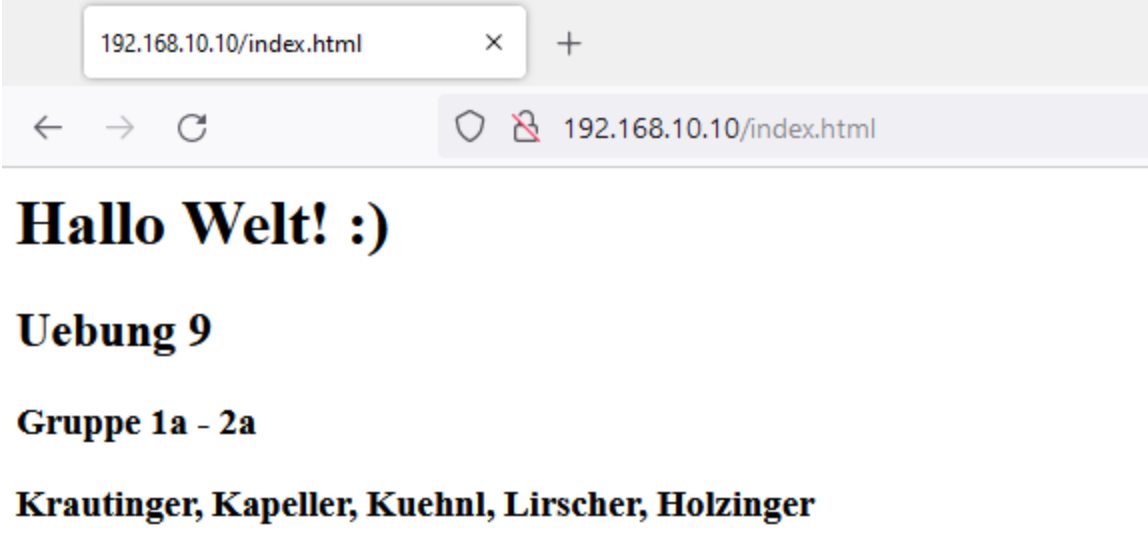
\includegraphics[scale=0.2]{screenshots/webserver_zugriff.png}
              \caption{Zugriff auf Webserver}
          \end{figure}
    \item Ping von PC2 auf PC3 (sollte NICHT\footnote{Funktioniert erst nach NAT-Konfiguration} funktionieren)
          \begin{figure}[H]
              \centering
              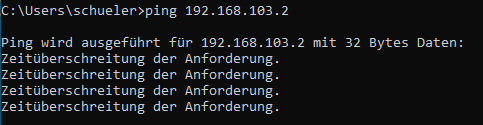
\includegraphics[scale=0.7]{screenshots/before nat.PNG}
              \caption{Ping PC2 $\rightarrow$ PC3 ohne NAT}
          \end{figure}
\end{itemize}

\section{NAT}
Laut Angabe soll NAT auf R1 und R2 konfiguriert werden. Weil dadurch der Service bei einem Tausch der Routerrollen (Active, Standby)
nicht mehr verfügbar wäre, haben wir uns gleich dazu entschieden NAT nur auf R3 zu konfigurieren. \\ \\
Wir sind bei der Konfiguration auf folgendes Problem gestoßen: das Netz zwischen R3 und R4 reicht mit einer Subnetzemaske
von /30 nicht aus. Deshalb haben wir dieses auf ein /24er-Netz geändert.

\subsection{Grundkonfiguration}
\begin{framed}
    \begin{verbatim}
        interface GigabitEthernet0/0/0
         ip nat inside
        !
        interface Serial0/1/0
         ip nat outside
        !
        interface Serial0/1/1
         ip nat inside
        !
        ip nat pool nat_VLAN20 192.168.101.3 192.168.101.10 netmask 
        255.255.255.0
        ip nat inside source list 1 pool nat_VLAN20
        ip route 192.168.10.0 255.255.255.0 192.168.102.1
        ip route 192.168.10.0 255.255.255.0 192.168.100.1 2
        ip route 192.168.20.0 255.255.255.0 192.168.102.1
        ip route 192.168.20.0 255.255.255.0 192.168.100.1 2
        !
        !
        access-list 1 permit 0.0.0.0 255.255.255.0
        access-list 1 permit 0.0.0.0 255.255.255.252
        access-list 1 permit 192.168.20.0 0.0.0.255
        access-list 1 permit 192.168.10.0 0.0.0.255
        !
    \end{verbatim}
\end{framed}

Die statischen Routen brauchen wir, weil R3 die VLANs 10 und 20 sonst nicht kennt.

\subsubsection{Überprüfung}
\begin{figure}[H]
    \centering
    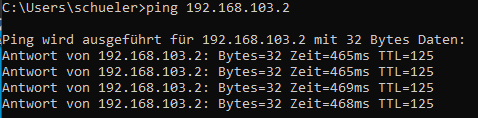
\includegraphics[scale=0.7]{screenshots/after nat.PNG}
    \caption{Ping PC2 $\rightarrow$ PC3 mit NAT}
\end{figure}

\subsection{Port Forwarding}
\begin{framed}
    \begin{verbatim}
        ip nat inside source static tcp 192.168.10.10 80 192.168.101.1 8080 
        extendable
    \end{verbatim}
\end{framed}

Somit ist der Port 80 (HTTP) vom Webserver auf Port 8080 in Local verfügbar.
\subsubsection{Überprüfung}
\begin{figure}[H]
    \centering
    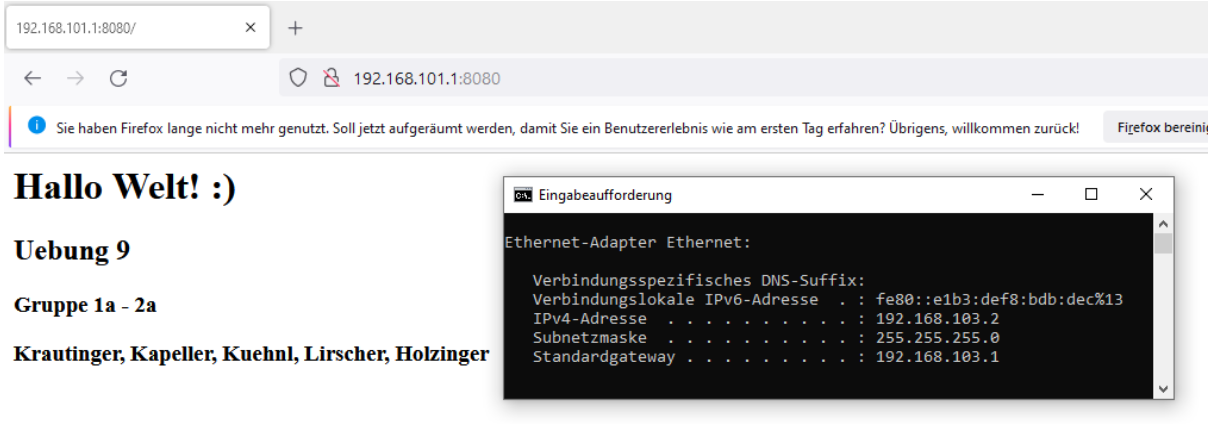
\includegraphics[scale=0.28]{screenshots/webserver_zugriff_port_forwarding.png}
    \caption{Zugriff auf Webserver mit Port Forwarding}
\end{figure}
\subsection{Überprüfung}
\begin{figure}[H]
    \centering
    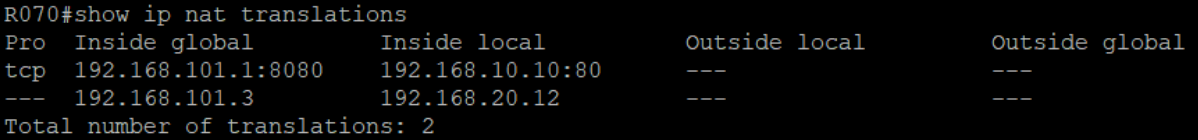
\includegraphics[scale=0.28]{screenshots/nat table.png}
    \caption{NAT Table}
\end{figure}

\section{HSRP/VRRP}
Die Protokolle HSRP oder VRRP lösen das "First-Hop-Problem". Dieses Problem tritt auf, wenn aufgrund des statisch
eingestellten First-Hop (Gateway) das Netz nicht mehr verfügbar ist. Mithilfe eines virtuellen Routers, der sich
auf den aktiven Routen "legt", ist immer ein verfügbarer First-Hop geboten (vorausgesetzt ist sind nicht alle
Router down).

\subsection{HSRP}
HSRP (Hot Standby Routing Protocol) ist das Protokoll von Cisco. Es wird unter Active und Standby-Routern unterschieden.
Diese Rollen können über die Priorität eingestellt werden. In unserem Fall ist R1 der Active Router im VLAN 10 und R2 der Active Router im VLAN 20.
\\ \\
Bei der Konfiguration haben wir dem Active Router in seinem $"$Active VLAN$"$ immer die Priorität 200 gegeben. Der Standby Router hingegen hat 100.
\\ \\
Geteilt:
\begin{itemize}
    \item VLAN 10
          \begin{itemize}
              \item Group-Number: 10
              \item Virtuelle IP: 192.168.10.254
          \end{itemize}
    \item VLAN 20
          \begin{itemize}
              \item Group-Number: 20
              \item Virtuelle IP: 192.168.20.254
          \end{itemize}
\end{itemize}
\subsubsection{Grundkonfiguration}
R1:
\begin{framed}
    \begin{verbatim}
        interface GigabitEthernet0/0/0.10
         standby 10 ip 192.168.10.254
         standby 10 priority 200
         standby 10 preempt
        !
        interface GigabitEthernet0/0/0.20
         standby 20 ip 192.168.20.254
         standby 20 preempt
        !    
    \end{verbatim}
\end{framed}

R2:
\begin{framed}
    \begin{verbatim}
        interface GigabitEthernet0/0/0.10
         standby 10 ip 192.168.10.254
         standby 10 preempt
        ! 
        interface GigabitEthernet0/0/0.20
         standby 20 ip 192.168.20.254
         standby 20 priority 200
         standby 20 preempt
        !
    \end{verbatim}
\end{framed}

$"$Preempt$"$ bedeutet, dass der ausgefallene ehemalige Active Router, wieder Active Router wird, sobald der Router wieder verfügbar ist.

\begin{figure}[H]
    \centering
    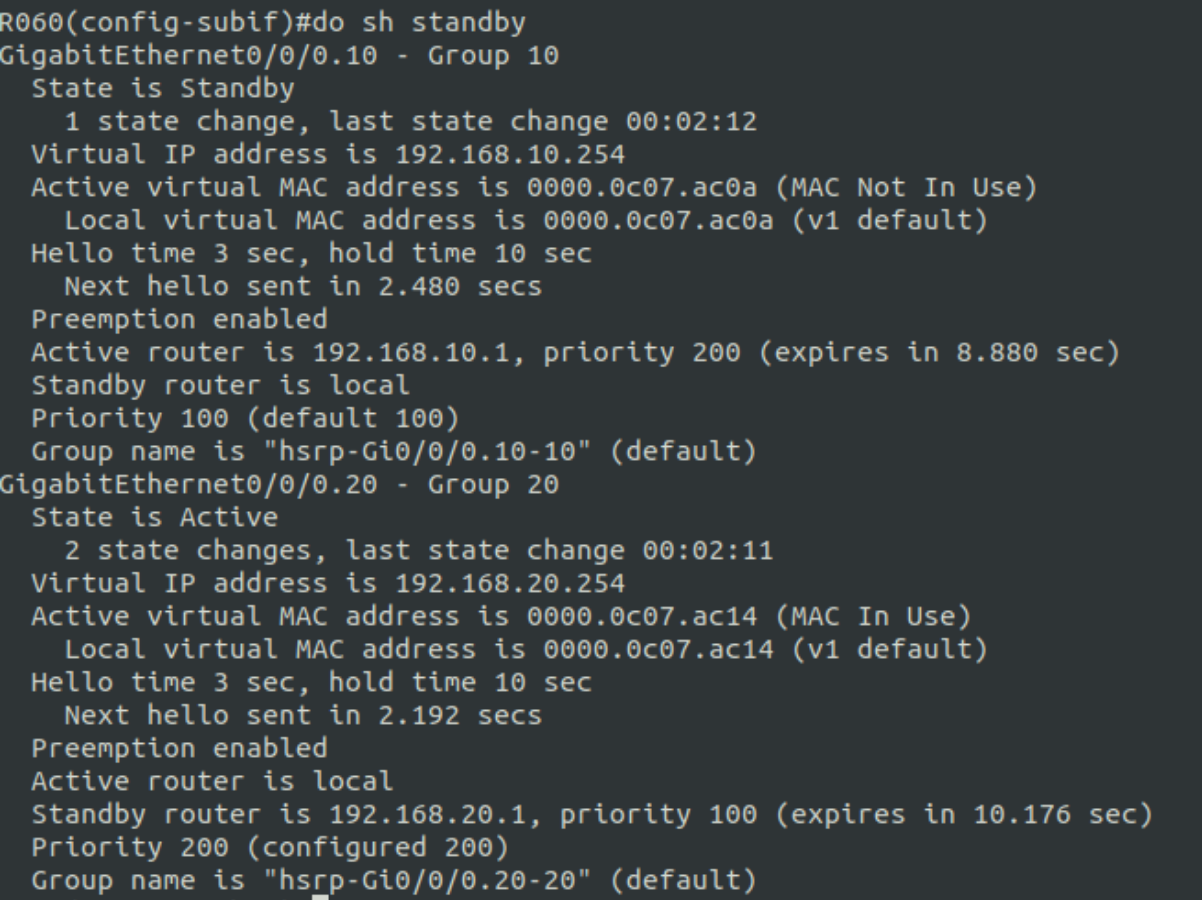
\includegraphics[scale=0.23]{screenshots/sh_standby before.png}
    \caption{HSRP-Konfiguration}
\end{figure}

\subsubsection{Object Tracking}
Object Tracking ist ein Konzept, um den Ausfall vom Link hinter dem Active Router zu regeln.
In unserem Fall soll fürs VLAN 10 beim Ausfall der Verbindung R1-R3, Router R2 der Active Router werden.
\\ \\
R1:
\begin{framed}
    \begin{verbatim}
        track 100 interface GigabitEthernet0/0/0.30 ip routing
        !
        interface GigabitEthernet0/0/0.10
         standby 10 track 100 decrement 200
        !
    \end{verbatim}
\end{framed}

Diese Konfiguration sagt aus, dass sobald das IP-Routing am Interface GigabitEthernet0/0/0.30 nicht mehr verfügbar ist,
die Priorität fürs VLAN 10 am Interface GigabitEthernet0/0/0.10 um 200 reduziert wird. Somit wird R2 Active Router.

Um dies zu testen, haben wir die Verbindung R1-R3 getrennt. Nach einer Zeit von 1-2 Pings, werden die Router umgeschalten.

\begin{figure}[H]
    \centering
    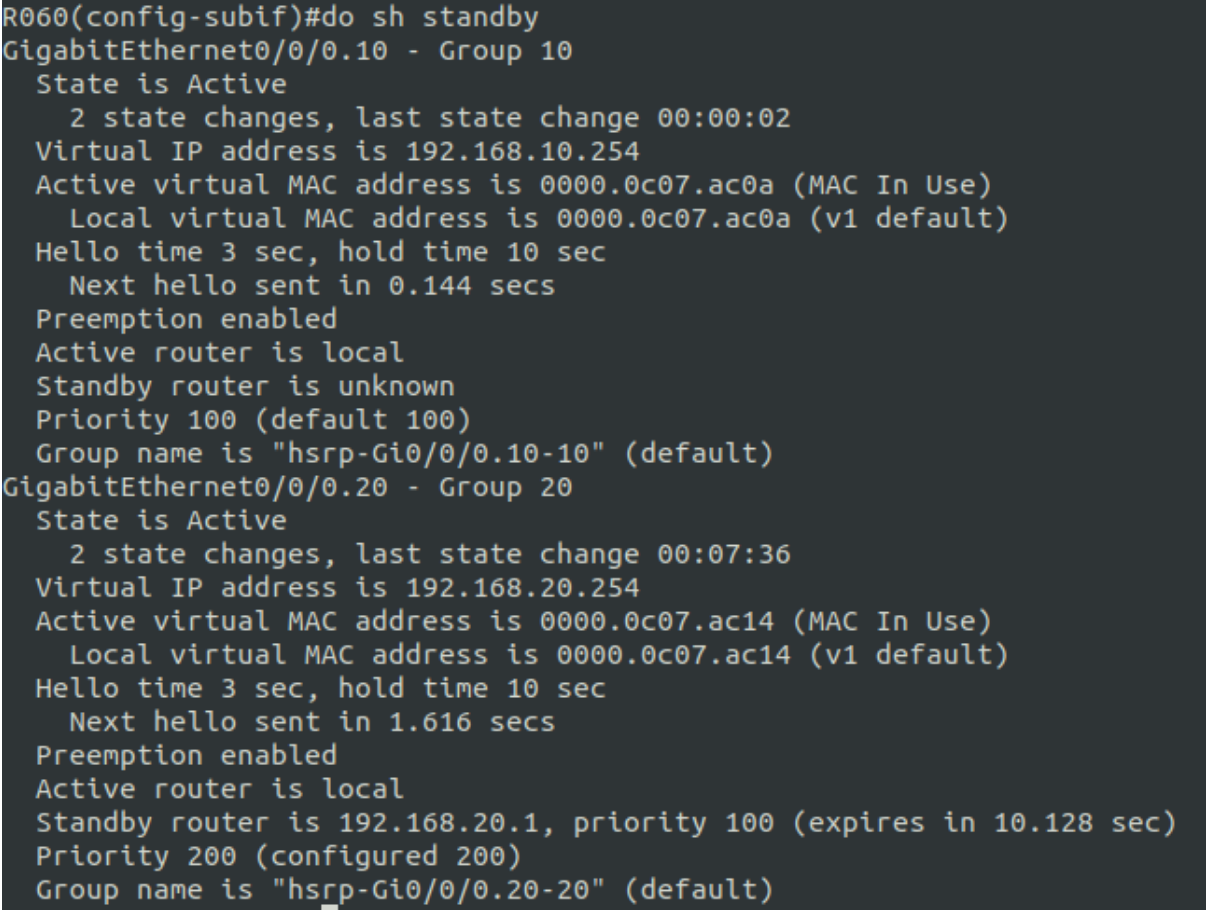
\includegraphics[scale=0.23]{screenshots/sh standby after.png}
    \caption{HSRP-Konfiguration ohne Verbindung R1-R3}
\end{figure}

\begin{figure}[H]
    \centering
    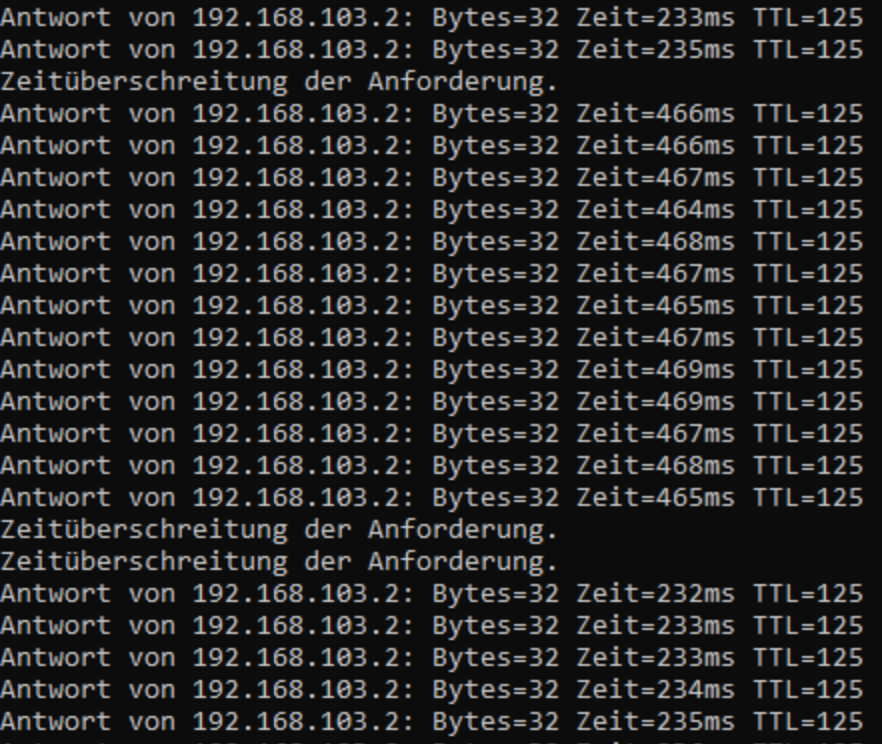
\includegraphics[scale=0.23]{screenshots/umschalten ping.png}
    \caption{Zeit für Umschalten}
\end{figure}

\subsection{VRRP}
VRRP verfolgt, die gleiche Idee wie HSRP, aber ist in der Konfiguration und den Details anders.
\\ \\
Der wichtigste Unterschied bei den Begriffen ist:
\begin{itemize}
    \item Active $\widehat{=}$ Master
    \item Standby $\widehat{=}$ Backup
\end{itemize}

\subsubsection{Konfiguration}
R1:
\begin{framed}
    \begin{verbatim}
        interface GigabitEthernet0/0/0.10
         vrrp 10 ip 192.168.10.250
         vrrp 10 priority 200
        !
        interface GigabitEthernet0/0/0.20
         vrrp 20 ip 192.168.20.250
        !
    \end{verbatim}
\end{framed}

R2:
\begin{framed}
    \begin{verbatim}
        interface GigabitEthernet0/0/0.10
         vrrp 10 ip 192.168.10.250
        !
        interface GigabitEthernet0/0/0.20
         vrrp 20 ip 192.168.20.250
         vrrp 20 priority 200
        !
    \end{verbatim}
\end{framed}

\end{document}